% Options for packages loaded elsewhere
\PassOptionsToPackage{unicode}{hyperref}
\PassOptionsToPackage{hyphens}{url}
\PassOptionsToPackage{dvipsnames,svgnames,x11names}{xcolor}
%
\documentclass[
]{article}

\usepackage{amsmath,amssymb}
\usepackage{iftex}
\ifPDFTeX
  \usepackage[T1]{fontenc}
  \usepackage[utf8]{inputenc}
  \usepackage{textcomp} % provide euro and other symbols
\else % if luatex or xetex
  \usepackage{unicode-math}
  \defaultfontfeatures{Scale=MatchLowercase}
  \defaultfontfeatures[\rmfamily]{Ligatures=TeX,Scale=1}
\fi
\usepackage{lmodern}
\ifPDFTeX\else  
    % xetex/luatex font selection
  \setmainfont[]{Latin Modern Roman}
  \setmathfont[]{Latin Modern Math}
\fi
% Use upquote if available, for straight quotes in verbatim environments
\IfFileExists{upquote.sty}{\usepackage{upquote}}{}
\IfFileExists{microtype.sty}{% use microtype if available
  \usepackage[]{microtype}
  \UseMicrotypeSet[protrusion]{basicmath} % disable protrusion for tt fonts
}{}
\makeatletter
\@ifundefined{KOMAClassName}{% if non-KOMA class
  \IfFileExists{parskip.sty}{%
    \usepackage{parskip}
  }{% else
    \setlength{\parindent}{0pt}
    \setlength{\parskip}{6pt plus 2pt minus 1pt}}
}{% if KOMA class
  \KOMAoptions{parskip=half}}
\makeatother
\usepackage{xcolor}
\setlength{\emergencystretch}{3em} % prevent overfull lines
\setcounter{secnumdepth}{5}
% Make \paragraph and \subparagraph free-standing
\ifx\paragraph\undefined\else
  \let\oldparagraph\paragraph
  \renewcommand{\paragraph}[1]{\oldparagraph{#1}\mbox{}}
\fi
\ifx\subparagraph\undefined\else
  \let\oldsubparagraph\subparagraph
  \renewcommand{\subparagraph}[1]{\oldsubparagraph{#1}\mbox{}}
\fi


\providecommand{\tightlist}{%
  \setlength{\itemsep}{0pt}\setlength{\parskip}{0pt}}\usepackage{longtable,booktabs,array}
\usepackage{calc} % for calculating minipage widths
% Correct order of tables after \paragraph or \subparagraph
\usepackage{etoolbox}
\makeatletter
\patchcmd\longtable{\par}{\if@noskipsec\mbox{}\fi\par}{}{}
\makeatother
% Allow footnotes in longtable head/foot
\IfFileExists{footnotehyper.sty}{\usepackage{footnotehyper}}{\usepackage{footnote}}
\makesavenoteenv{longtable}
\usepackage{graphicx}
\makeatletter
\def\maxwidth{\ifdim\Gin@nat@width>\linewidth\linewidth\else\Gin@nat@width\fi}
\def\maxheight{\ifdim\Gin@nat@height>\textheight\textheight\else\Gin@nat@height\fi}
\makeatother
% Scale images if necessary, so that they will not overflow the page
% margins by default, and it is still possible to overwrite the defaults
% using explicit options in \includegraphics[width, height, ...]{}
\setkeys{Gin}{width=\maxwidth,height=\maxheight,keepaspectratio}
% Set default figure placement to htbp
\makeatletter
\def\fps@figure{htbp}
\makeatother

\usepackage{arxiv}
\usepackage{orcidlink}
\usepackage{amsmath}
\usepackage[T1]{fontenc}
\makeatletter
\@ifpackageloaded{caption}{}{\usepackage{caption}}
\AtBeginDocument{%
\ifdefined\contentsname
  \renewcommand*\contentsname{Table of contents}
\else
  \newcommand\contentsname{Table of contents}
\fi
\ifdefined\listfigurename
  \renewcommand*\listfigurename{List of Figures}
\else
  \newcommand\listfigurename{List of Figures}
\fi
\ifdefined\listtablename
  \renewcommand*\listtablename{List of Tables}
\else
  \newcommand\listtablename{List of Tables}
\fi
\ifdefined\figurename
  \renewcommand*\figurename{Figure}
\else
  \newcommand\figurename{Figure}
\fi
\ifdefined\tablename
  \renewcommand*\tablename{Table}
\else
  \newcommand\tablename{Table}
\fi
}
\@ifpackageloaded{float}{}{\usepackage{float}}
\floatstyle{ruled}
\@ifundefined{c@chapter}{\newfloat{codelisting}{h}{lop}}{\newfloat{codelisting}{h}{lop}[chapter]}
\floatname{codelisting}{Listing}
\newcommand*\listoflistings{\listof{codelisting}{List of Listings}}
\makeatother
\makeatletter
\makeatother
\makeatletter
\@ifpackageloaded{caption}{}{\usepackage{caption}}
\@ifpackageloaded{subcaption}{}{\usepackage{subcaption}}
\makeatother
\ifLuaTeX
  \usepackage{selnolig}  % disable illegal ligatures
\fi
\IfFileExists{bookmark.sty}{\usepackage{bookmark}}{\usepackage{hyperref}}
\IfFileExists{xurl.sty}{\usepackage{xurl}}{} % add URL line breaks if available
\urlstyle{same} % disable monospaced font for URLs
\hypersetup{
  colorlinks=true,
  linkcolor={blue},
  filecolor={Maroon},
  citecolor={Blue},
  urlcolor={Blue},
  pdfcreator={LaTeX via pandoc}}

\newcommand{\runninghead}{A Preprint }
\def\asep{\\\\\\ } % default: all authors on same column
\author{}
\date{}
\begin{document}
\section*{Supplementary material}\label{supplementary-material}
\addcontentsline{toc}{section}{Supplementary material}

\renewcommand{\thetable}{\roman{table}}
\renewcommand{\thefigure}{\roman{figure}}

\emph{Overture data product attributes}

\def\arraystretch{1.5}
\begin{table}[H]
\caption{\label{tablei} Attributes in Overture UK open data product, with an additional indicator describing which attributes were processed out of their nested JSON format.}
\centering
\bigskip
\begin{tabular}{p{6cm}p{6cm}c}
\hline
\multicolumn{1}{c}{\textbf{Attribute}}                                                                        & \multicolumn{1}{c}{\textbf{Description}}                                                                     & \textbf{Processed} \\
\hline
id                                                                                                   & Unique ID assigned by Overture.                                                                     & N         \\
updatetime, version                                                                                  & Information about the version (and date) of the Overture data - most recent.                        & N         \\
confidence                                                                                           & Attribute assigned by Overture                                                                      & N         \\
websites, socials, emails, phones                                                                    & Contact information and social media associated with POI.                                           & N         \\
names\_value                                                                                         & POI name.                                                                                           & Y         \\
category\_main, category\_alternative                                                                & Assigned category for POI.                                                                          & Y         \\
addresses\_postcode, addresses\_freeform, addresses\_country, addresses\_locality, addresses\_region & Address information for POI.                                                                        & Y         \\
sources\_dataset                                                                                     & Data source (meta or microsoft)                                                                     & N         \\
lat, lng                                                                                             & Coordinates for POI.                                                                                & N         \\
h3\_01 ... h3\_09                                                                                    & H3 addresses for each POI.                                                                          & N         \\
easting, northing                                                                                    & Coordiantes for POI.                                                                                & N         \\
LAD22CD ... LGD2014\_nm                                                                              & Administrative geographies for each POI, different for England/Wales, Scotland and Northern Ireland & N         \\
\hline
\end{tabular}
\end{table}

\emph{Scraping Overture data for specific brands}

As discussed in the main body, extracting a complete list of POIs for a
brand (e.g., Waitrose) is difficult due to missing values in the
category and brand columns. For example, selecting all POIs by brand, as
below in Figure i, results in 0 POIs for Waitrose, and 1,934 POIs for
Spar.

\begin{figure}[H]

{\centering 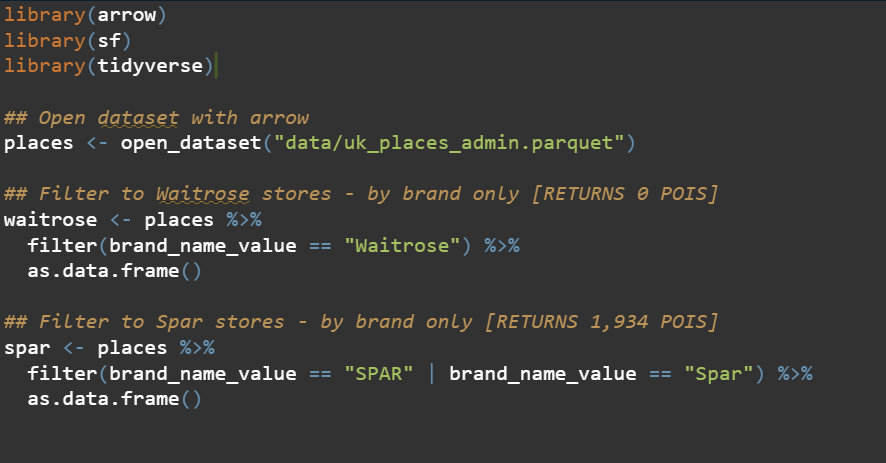
\includegraphics{./figures/figure2.png}

}

\caption{R code snippet highlighting brand filtering of POIs.}

\end{figure}%

However, by integrating additional filters, specifically on the POI name
and the POI category columns, you can get to the final list of POIs for
each retail brand, which closely resemble those in the Geolytix dataset.
For example, in Figure ii we show that the brand and name columns need
to be filtered to extract all Spar supermarket stores, and name and
category columns need to be filtered to extract all Waitrose
supermarkets (excluding petrol stations and other retail formats). This
code snippet (Figure ii) results in 420 POIs for Waitrose, and 2,308
POIs for Spar, as in Table 1. This has strong implications for future
use of this dataset, where users should consider POI name, brand and
category if seeking to extract a complete list of POIs for specific
research questions or applications.

\begin{figure}[H]

{\centering 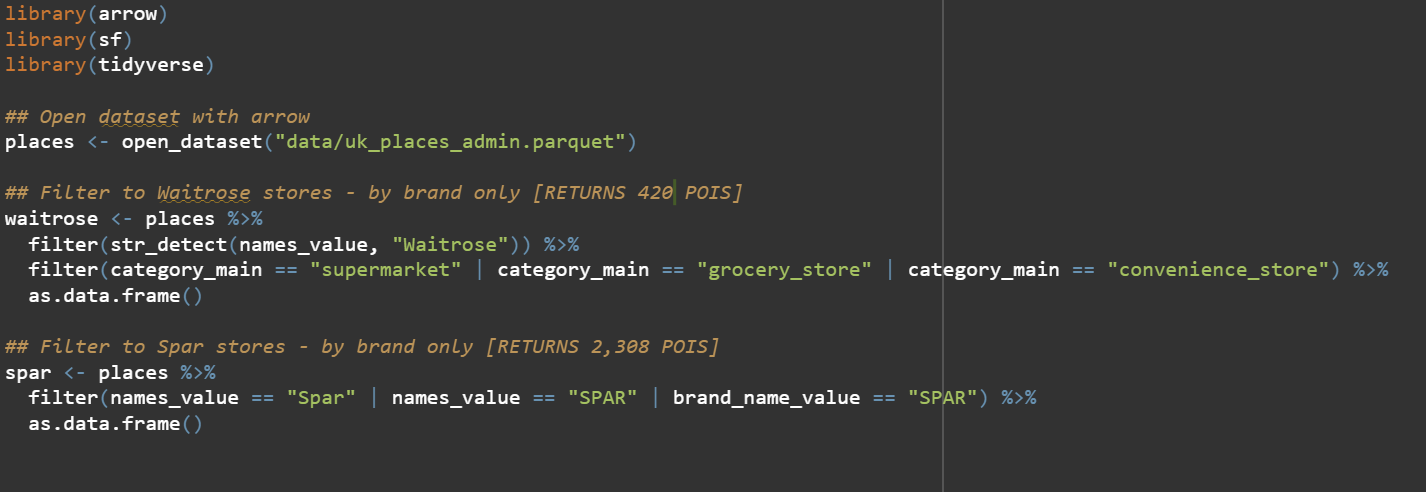
\includegraphics{./figures/figure3.png}

}

\caption{Code snippet highlighting additional filtering of POI
attributes.}

\end{figure}%



\end{document}
